\chapter{A Simulator for Joint Source-Channel Codes}%

\DefineShortVerb{\|}

Just a citation so that \LaTeX\ doesn't complain~\cite{KleinerR2009}.

\section{Introduction}

This section introduces the simulator and explains why the object-oriented
programming paradigm, especially inheritance, is particularly suited for the
task of simulating many similar communication strategies.

There are two main advantages to the object-oriented approach. The first is the
ability to quickly produce an alternative version of a scheme with only small
changes, without the need to copy a complete file or modify the original. This
is demonstrated by the many variations of a quantize/uncoded scheme. The second
advantage is that the code to run and to evaluate the results of the many
schemes need only be written one for a shared interface. 


\section{A Step-By-Step Tutorial}

\paragraph{Theoretical Performance}
The first thing one might like to do when studying a new joint source-channel
code is to compare its performance to the theoretical optimum. To this end,
let us create a ``virtual'' or ``theoretical'' communication scheme, \ie, one
that does not actually do any coding, but simply returns a theoretical error
value given the SNR.

\begin{listing}
\begin{Code}
  classdef ShannonScheme < Scheme
    properties
      n         % The number of channel uses per source symbol.
    end

    methods
      function obj = ShannonScheme(sv, s, n)
        
        % Call base class constructor.
        obj = obj@Scheme(sv, s);

        % Set class-specific parameters.
        obj.n = n;
      end

      % This function simply returns the theoretically optimal MSE
      % for the SNR.
      function mse = compute_mse(obj)
        mse = obj.sv / (1 + obj.snr)^obj.n;
      end
    end
  end
\end{Code}
  \caption{A ``theoretical'' communication scheme that does not perform any
  actual encoding or decoding, but rather computes the theoretically optimal MSE
  for a given SNR.}
  \label{lst:shannonscheme}
\end{listing}

The resulting \matlab\ code is given in \lstref{shannonscheme}. We can make the
following observations.
\begin{enumerate}
  \item The line |classdef ShannonScheme < Scheme| defines a new class
    called |ShannonScheme| and specifies that it is derived from the
    \emph{base class} |Scheme|. This is the class from which all communication
    schemes must be derived; the only requirement it puts is that any derived
    class must implement a function |compute_mse()| that returns the mean
    squared error obtained for a given SNR.

  \item The class |ShannonScheme| has a single parameter, namely the number~|n|
    of channel uses per source symbol.

  \item The first function in the |methods| block, called |ShannonScheme()|, is
    the \emph{constructor} of the class. It is called automatically when a new
    instance of the class is created. The main job of the constructor is to call
    the constructor of the base class and save class-specific parameters that
    are specified when the class is created, in this case the
    parameter~|n|.\footnote{If you wonder why the constructor returns something
    called \Verb+obj+: this is simply how \matlab's syntax specifies the
    constructor.  The returned value stands for the object just created, and it
    serves as a ``pointer'' to access the object's properties, similar to the
    \Verb+this+ keyword in C++ or Java.}

  \item The second function, |compute_mse(obj)|, is the heart of this class. It
    computes the formula $\text{MSE} = \ssq / (1 + \snr)^n$. To access any of
    the class properties, their name must be prefixed by `|obj.|'.
    Note in particular how |obj.snr| is accessed, even though it was never
    defined within this class. This is because it is handled by the base class. 
\end{enumerate}


\paragraph{Performance Analysis}
Having implemented the class |ShannonScheme|, the next thing one might like to
do is to plot the resulting performance. This task is much simplified by the
class |PerformanceProcessor|, which is used as follows.
\CodeInput{figures/matlab/ex_shannonscheme.minc}
The first two lines define two \emph{cell arrays} with each a single entry.
|schemes| contains the class names of the schemes to plot, and |parameters|
contains a list of parameters for each scheme. Here we only have a single
scheme, |ShannonScheme|, and we would like to plot its performance for $n = 1$,
$2$, and~$3$. The third line creates an instance of the class
|PerformanceProcessor|, whose |plot_performance()| method is invoked in the
fourth line, specifying the relevant schemes and parameters. The resulting plot
is shown on \figref{shannonschemeperf}.

\begin{figure}
  \begin{center}
    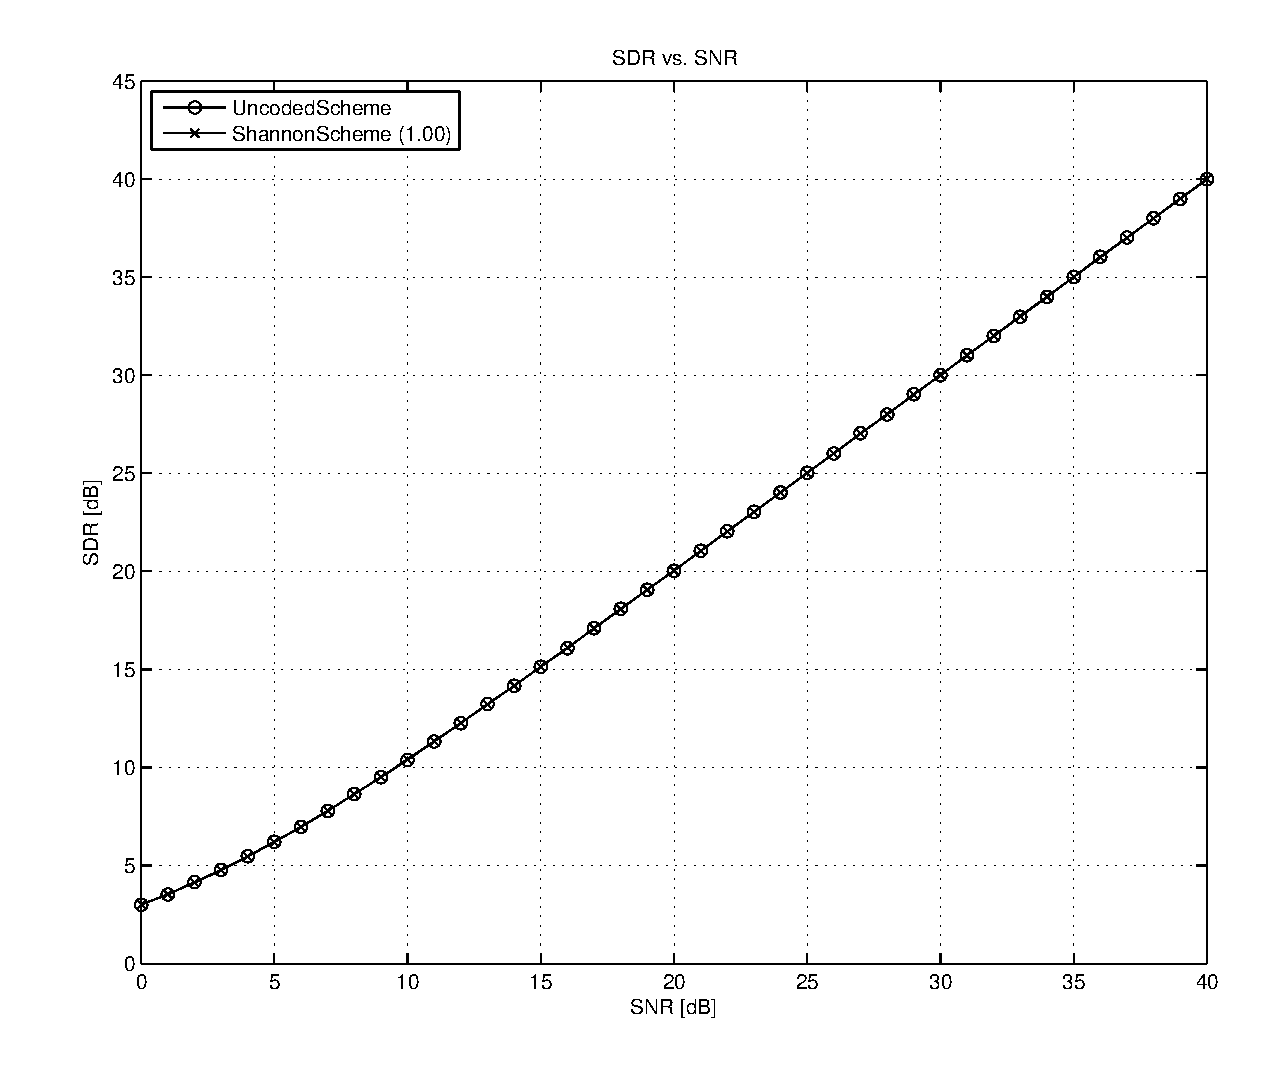
\includegraphics[width=\textwidth]{figures/matlab/ex_shannonscheme.pdf}
  \end{center}
  \caption{Plot of the SDR resulting from the \texttt{ShannonScheme} class,
  obtained using a \texttt{PerformanceProcessor}.}
  \label{fig:shannonschemeperf}
\end{figure}


\paragraph{Implementing a Practical Scheme}
The communication scheme just implemented only computed theoretical performance
results; nothing was actually simulated. Let us then move ahead and create an
actual, practically implementable scheme. To start, \lstref{uncoded} shows an
implementation of ``uncoded'' communication, which was shown in \chapref{prelim}
to be optimal.

\begin{listing}
  \CodeInput{simulator/@UncodedScheme/UncodedScheme.m}
  \caption{Implementation of uncoded transmission.}
  \label{lst:uncoded}
\end{listing}

We can make the following observations.
\begin{enumerate}
  \item The class is derived from |PracticalScheme|, rather than |Scheme|.
    |PracticalScheme| is the base class for all ``practical'' schemes, \ie,
    actually implementable ones (as the name says).

  \item The constructor receives two parameters. |sv| is the source variance and
    |s| is the sequence of source symbols that are to be transmitted. These
    two parameters are the same for all communication schemes involved in a
    simulation; this ensures that a fair comparison can be made. 

    The constructor of |PracticalScheme| needs two additional parameters. They
    are, respectively, the number~$k$ of source symbols at a time and the
    number~$n$ of channel inputs produced from every $k$~source symbols. The
    scheme at hand works only for the particular case when~$k = n = 1$, which is
    why the last two parameters passed to |PracticalScheme()| are both~$1$.

  \item The actual work of the class is done by the functions |encode()| and
    |decode()|. Any class derived from |PracticalScheme| \emph{must} implement
    these functions. Here they simply compute $X = \sqrt{P/\ssq} S$ and $\Sh =
    \sqrt{P \ssq} Y / (P + \szq)$.
\end{enumerate}

To verify the result from \chapref{prelim} that uncoded transmission is optimal
for $k=n=1$, let us now plot the performance of the communication scheme just
implemented, together with the theoretically optimal performance for $n = 1$ and
$n=2$. 
\CodeInput{figures/matlab/ex_uncoded.minc}
The only difference to the previous example is that here the list of schemes is
augmented by |UncodedScheme|, and an empty vector is added in the corresponding
position of the parameter list (since |UncodedScheme| has no parameters). 
The output is shown on \figref{uncoded}; indeed, the SDR curve of
|UncodedScheme| coincides exactly with that of |ShannonScheme| for $n = 1$.

\begin{figure}
  \begin{center}
    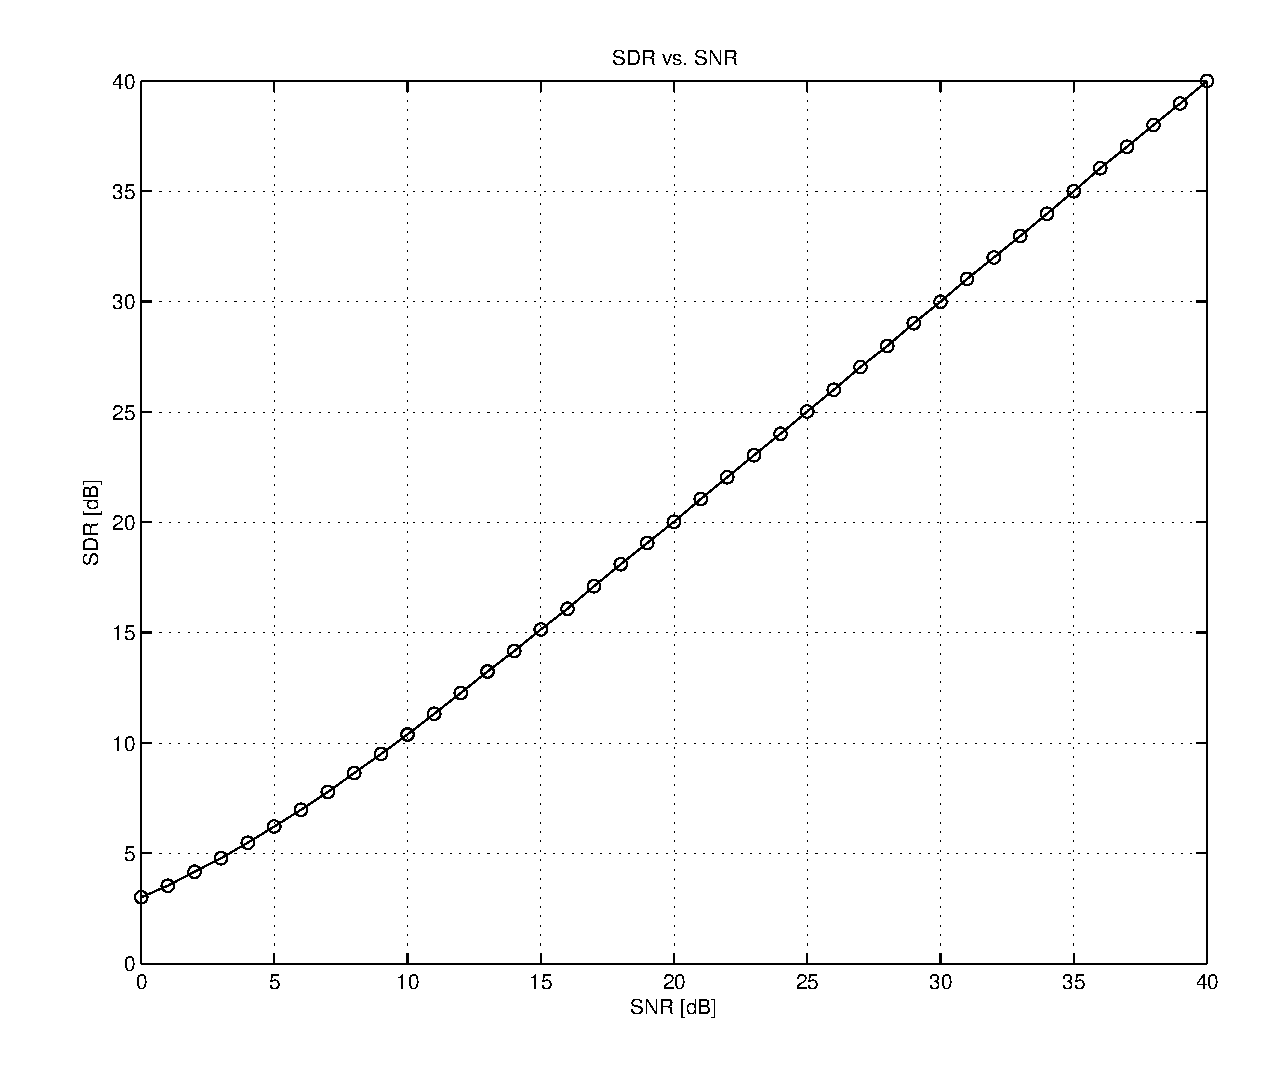
\includegraphics[width=\textwidth]{figures/matlab/ex_uncoded.pdf}
  \end{center}
  \caption{The performance of uncoded transmission for $n=1$. It is clearly
  visible that the theoretical optimum is achieved.}
  \label{fig:uncoded}
\end{figure}

Let us summarize what we have done so far:
\begin{enumerate}
  \item We have created a ``theoretical'' communication scheme that computes the
    theoretically optimal MSE for a bandwidth expansion factor~$n$.

  \item We have implemented uncoded transmission by essentially writing the
    |encode()| and |decode()| functions of the class |UncodedScheme|.

  \item To plot the performance, we have passed a list of communication schemes
    along with the respective parameters to a |PerformanceProcessor| object.
\end{enumerate}
This looks like not much at all. Behind the scenes, however, a lot more was
going on:
\begin{enumerate}
  \item A long sequence of random source symbols were generated.
  \item For a range of SNR values and for each communication scheme, the source
    sequence was encoded using the communication scheme, Gaussian noise of the
    appropriate variance was added, and the result was decoded using the
    scheme's |decode()| function.
  \item The average difference between the source sequence and the estimate
    sequence was computed, again for each scheme and for each value of SNR. 
  \item The resulting performance curves were plotted by |plot_performance()|.
\end{enumerate}
All this work is encapsulated in the class structure, leaving you free to focus
on the essential stuff.


\paragraph{Alternative Output Formats}
So far, the call to |plot_performance()| just created a standard \matlab\ figure
window containing the performance plot. Often, though, you may not only want to
look at the plot on the screen but also use it in some other document, like a
report or a paper. For this, there is the concept of \emph{output module}. An
output module defines a rudimentary set of plot capabilities. The default output
module uses \matlab's plot command to display a figure window. Alternatively,
suppose you want to save the performance plot in a PDF file. For this you can
use the default output module, which is called |MatlabPlotModule|, by one called
|MatlabFilePlotModule|. Instead of displaying the plot in a window, it saves it
in a file. Continuing our previous example, we would use it as follows.
\begin{Code}
  ...  % Define list of schemes and parameters.
  pp = PerformanceProcessor();
  om = MatlabFilePlotModule();
  om.fn = 'myplot.pdf';
  pp.om = om;
  pp.plot_performance(schemes, parameters);  % Saved to myplot.pdf.
\end{Code}
In the second line, a new output module of type |MatlabFilePlotModule| is
created. Since it writes its output to a file, we have to specify a file name,
which we do in the next line. Finally, in the fourth line, we replace the
default output module of the performance processor with newly created
one.\footnote{Unsurprisingly, Figures~\ref{fig:shannonschemeperf}
and~\ref{fig:uncoded} have been created using \Verb+MatlabFilePlotModule+.}

Another output module is called |PGFPlotsOutputModule|. It produces a file
containing \TeX\ code, to be used with the \pgfplots\ package. To use it, just
replace |MatlabFilePlotModule| in the above example by |PGFPlotsOutputModule|
and set \eg
\begin{Code}
  om.fn = 'myplot.tex';
\end{Code}
The file |myplot.tex| can then be included in a \LaTeX\ file using the |\input|
command, provided that the |pgfplots| package has been loaded.  The result is
shown on \figref{uncodedpgf}. Admittedly, the plot created by \pgfplots\ fits in
nicer with the \LaTeX\ layout.

\begin{figure}
  \begin{center}
    \input{figures/matlab/ex_uncodedpgf.tex_t}
  \end{center}
  \caption{The same plot as that in \figref{uncoded}, but here a
  \texttt{PGFPlotsOutputModule} was used instead.}
  \label{fig:uncodedpgf}
\end{figure}


\section{Class Hierarchy and Reference}

\subsection{Communication Strategies}

\subsection{Processors}

\subsection{Output}

\subsection{Batch Processing and Makefile Inclusion}


\section{Implementation Notes}
